\section{景观诊断与综合分析}\label{sec:landscape}

\begin{chapterquestion}
\textbf{本章研究的问题}：前述异常现象能否得到一致性的解释？
\end{chapterquestion}

本节对前述现象进行综合分析。需要界定其定位：
它不是孤立分析，而是为第~\ref{sec:anomaly}--\ref{sec:converge}~节的异常现象
提供一种一致性的解释框架；它是本文当前\emph{最有说服力的解释}，
而非唯一支柱——其结论也可被"数据覆盖不足、OOD 效应、数据流形约束、
共线性结构"等同源机制部分替代（见第~\ref{subsec:counterfactual}~小节）。

\subsection{核心问题：优化器失效还是景观退化？}

前述异常可归结为一个判别性问题：
解的趋同，源于\emph{优化器搜索失败}，还是\emph{目标函数景观退化}？
本节从两条路径分析：一是诊断代理对参数的敏感性与数据结构
（第~\ref{subsec:wing-sens}--\ref{subsec:data-struct}~小节），
二是通过新增的去饱和实验进行机制验证（第~\ref{subsec:desat}~小节）。

\subsection{代理对参数的敏感性}\label{subsec:wing-sens}

\begin{figure}[H]
\centering
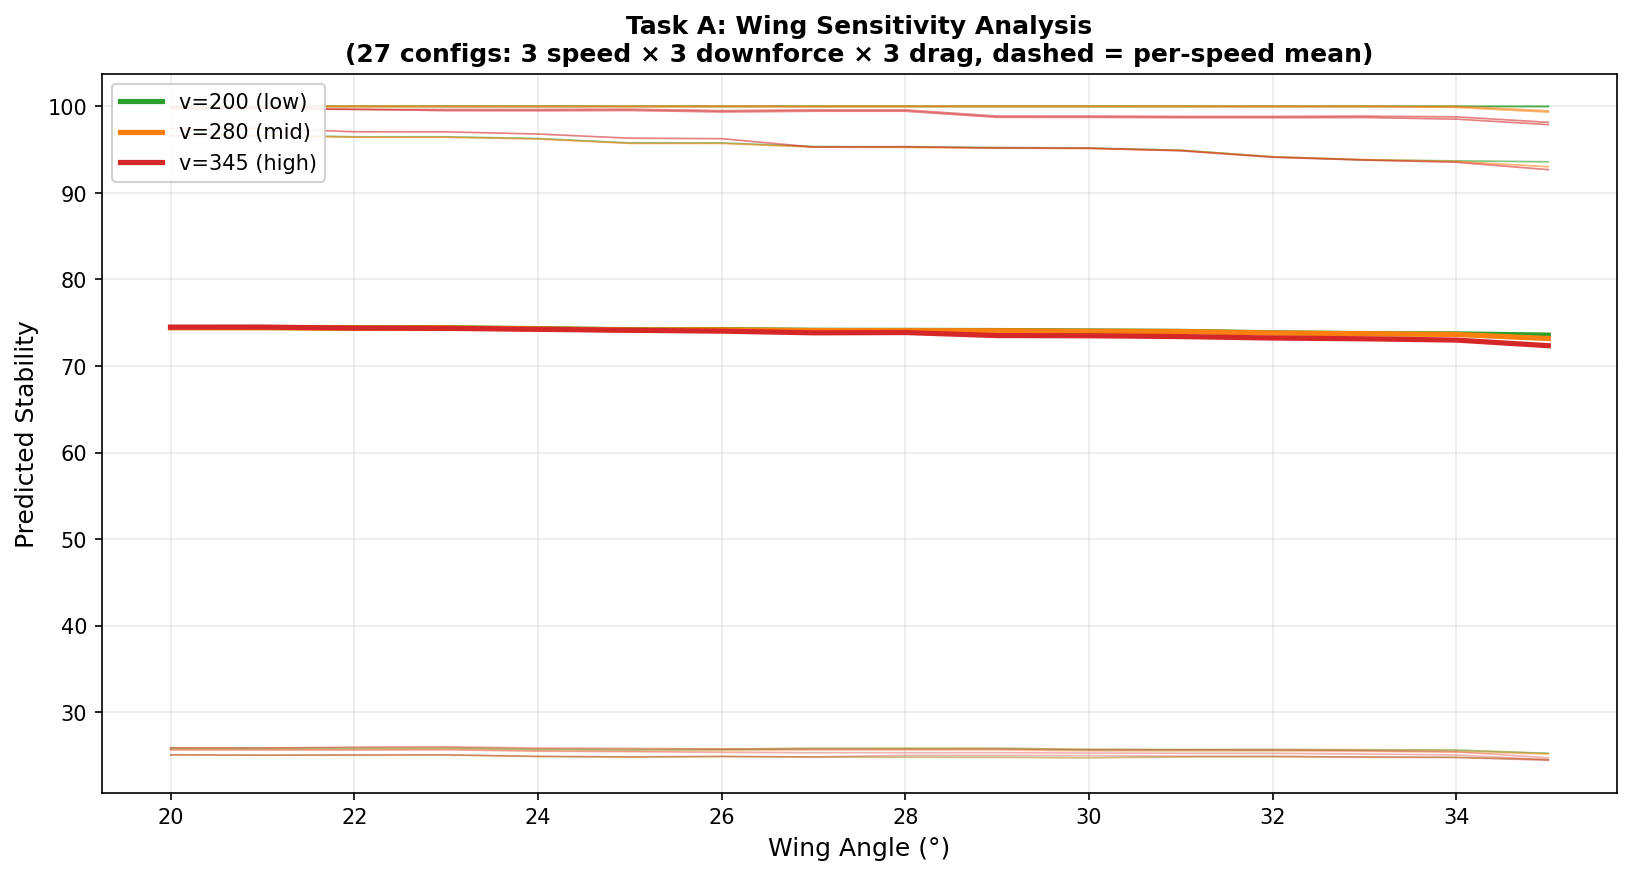
\includegraphics[width=0.78\textwidth]{figures/diagnosis_wing_sensitivity.png}
\caption{翼角敏感性扫描结果}
\label{fig:wing_sens}
\end{figure}

对 XGBoost 做翼角敏感性扫描（27 组固定配置，wing $20^\circ\to35^\circ$）显示：
模型能够感知 wing——在 345 km/h 下最大 $\Delta\text{Stability}=2.15$（斜率 $-0.126$/度），
$\text{wing}\uparrow\Rightarrow\text{stability}\downarrow$ 的关系被正确学习。
需要指出的是：这些可感知的变化发生在 stability $72$--$74$ 的非饱和区；
而 PSO 找到的最优配置处 stability $\approx100$（饱和区），
wing 的变化不再产生可辨影响。

\begin{figure}[H]
\centering
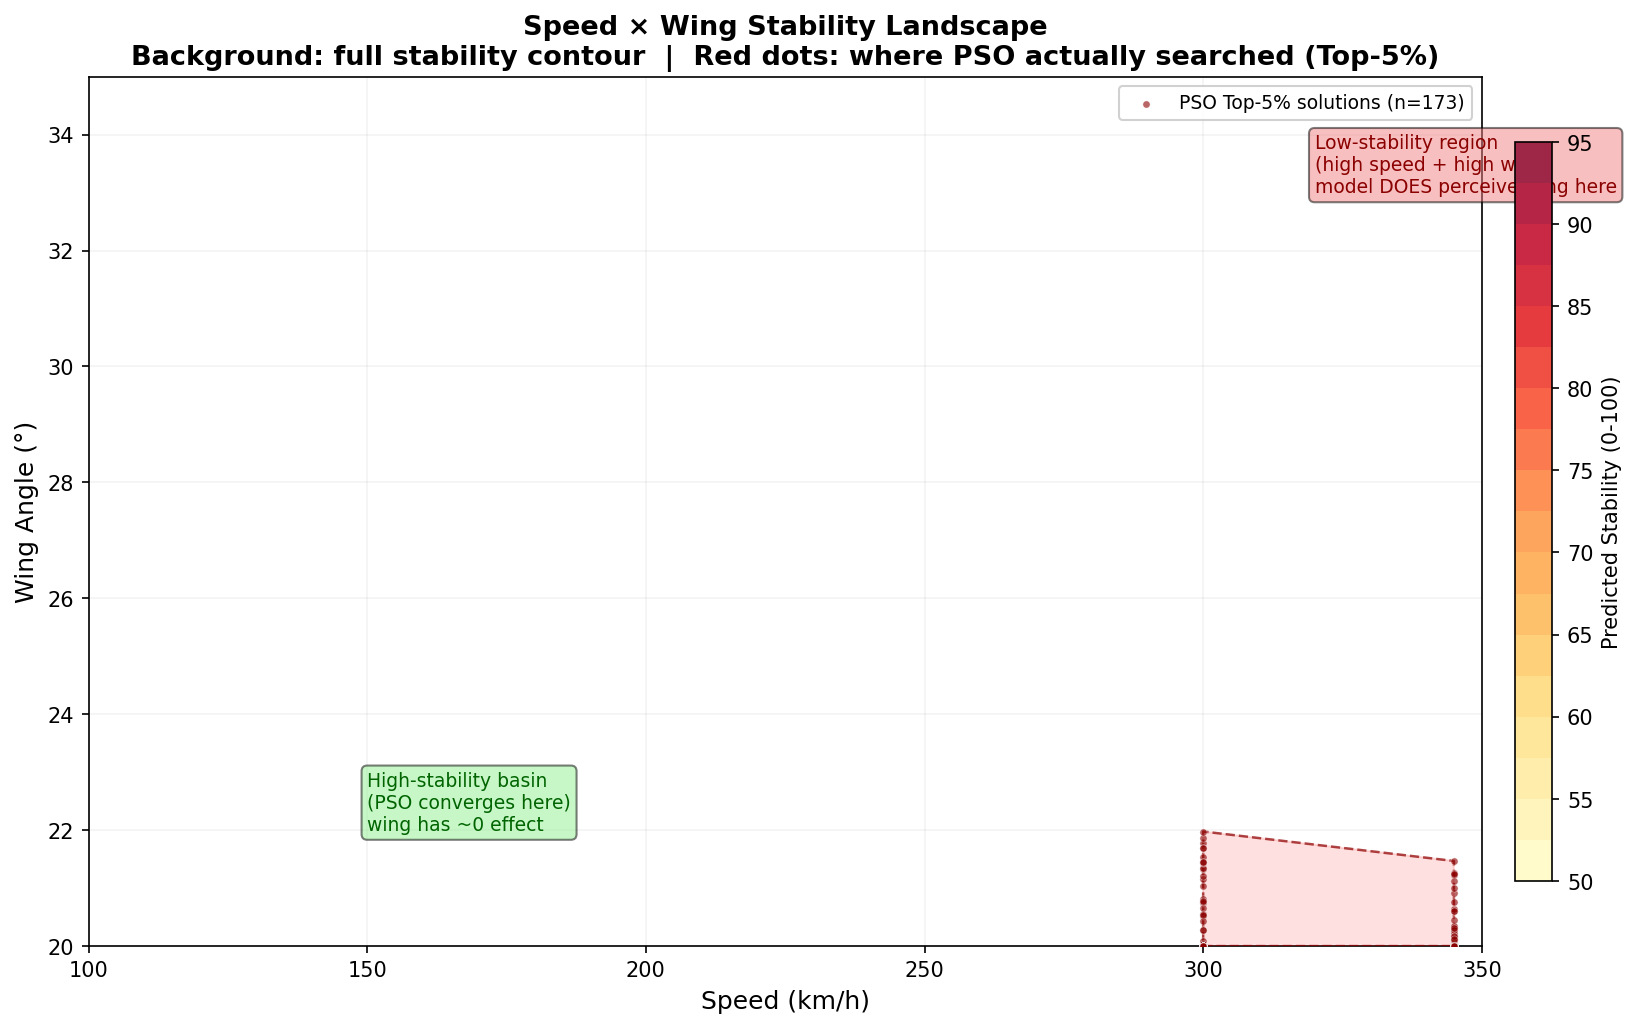
\includegraphics[width=0.90\textwidth]{figures/diagnosis_speed_wing_pso_overlay.png}
\caption{Speed$\times$Wing 稳定性等高线与 PSO 解的叠加}
\label{fig:overlay}
\end{figure}

图~\ref{fig:overlay} 在同一坐标内同时呈现三点：
① 模型感知 wing——右下角（高速$+$大翼角）等高线可测量地下沉（梯度峰值 $0.63$）；
② PSO 避开了低稳定区——Top-5\% 解集中在左上角的高稳定盆地；
③ 高稳定盆地内等高线近乎水平——wing 从 $20^\circ$ 到 $35^\circ$ 几乎不改变预测。
据此可以判断：wing$\to20^\circ$ 是模型在饱和盆地内的数学正确解，而非 PSO 搜索缺陷；
PSO 并非无法识别 wing 的影响，而是避开了 wing 有影响但稳定性更低的区域。

\subsection{数据结构层面的来源}\label{subsec:data-struct}

盆地平坦的来源可追溯到数据结构：
\begin{itemize}
    \item \textbf{偏相关}：控制 downforce 后，wing 与 stability 的偏相关仅 $r=0.06$，
        wing 的影响几乎全经 downforce 中介，一旦 downforce 被锁定，wing 即成冗余变量；
    \item \textbf{互信息}：$\text{MI(downforce, stability)}=1.25$ 占主导，
        $\text{MI(wing, stability)}=0.14$ 仅为前者的 $11\%$；
    \item \textbf{SHAP 与排列重要性}（作为辅助解释，见第~\ref{subsec:shap}~小节）：
        downforce 贡献约 $96\%$，打乱 downforce 后 $R^2$ 下降 $1.88$，其余特征影响较小。
\end{itemize}
叠加第~\ref{sec:dataset}~节的两项结构特征（86\% 饱和、downforce$\leftrightarrow$drag $r=0.895$ 共线），
目标在高稳定区接近退化为 $\text{stability}\approx f(\text{downforce})$ 的单变量函数。

\subsection{去饱和实验：机制验证（新增）}\label{subsec:desat}

上述诊断为相关性分析。为进行机制验证，本文新增去饱和实验：
对（饱和的）稳定性目标施加不同变换后重新寻优，观察最优解是否移动。

\begin{figure}[H]
\centering
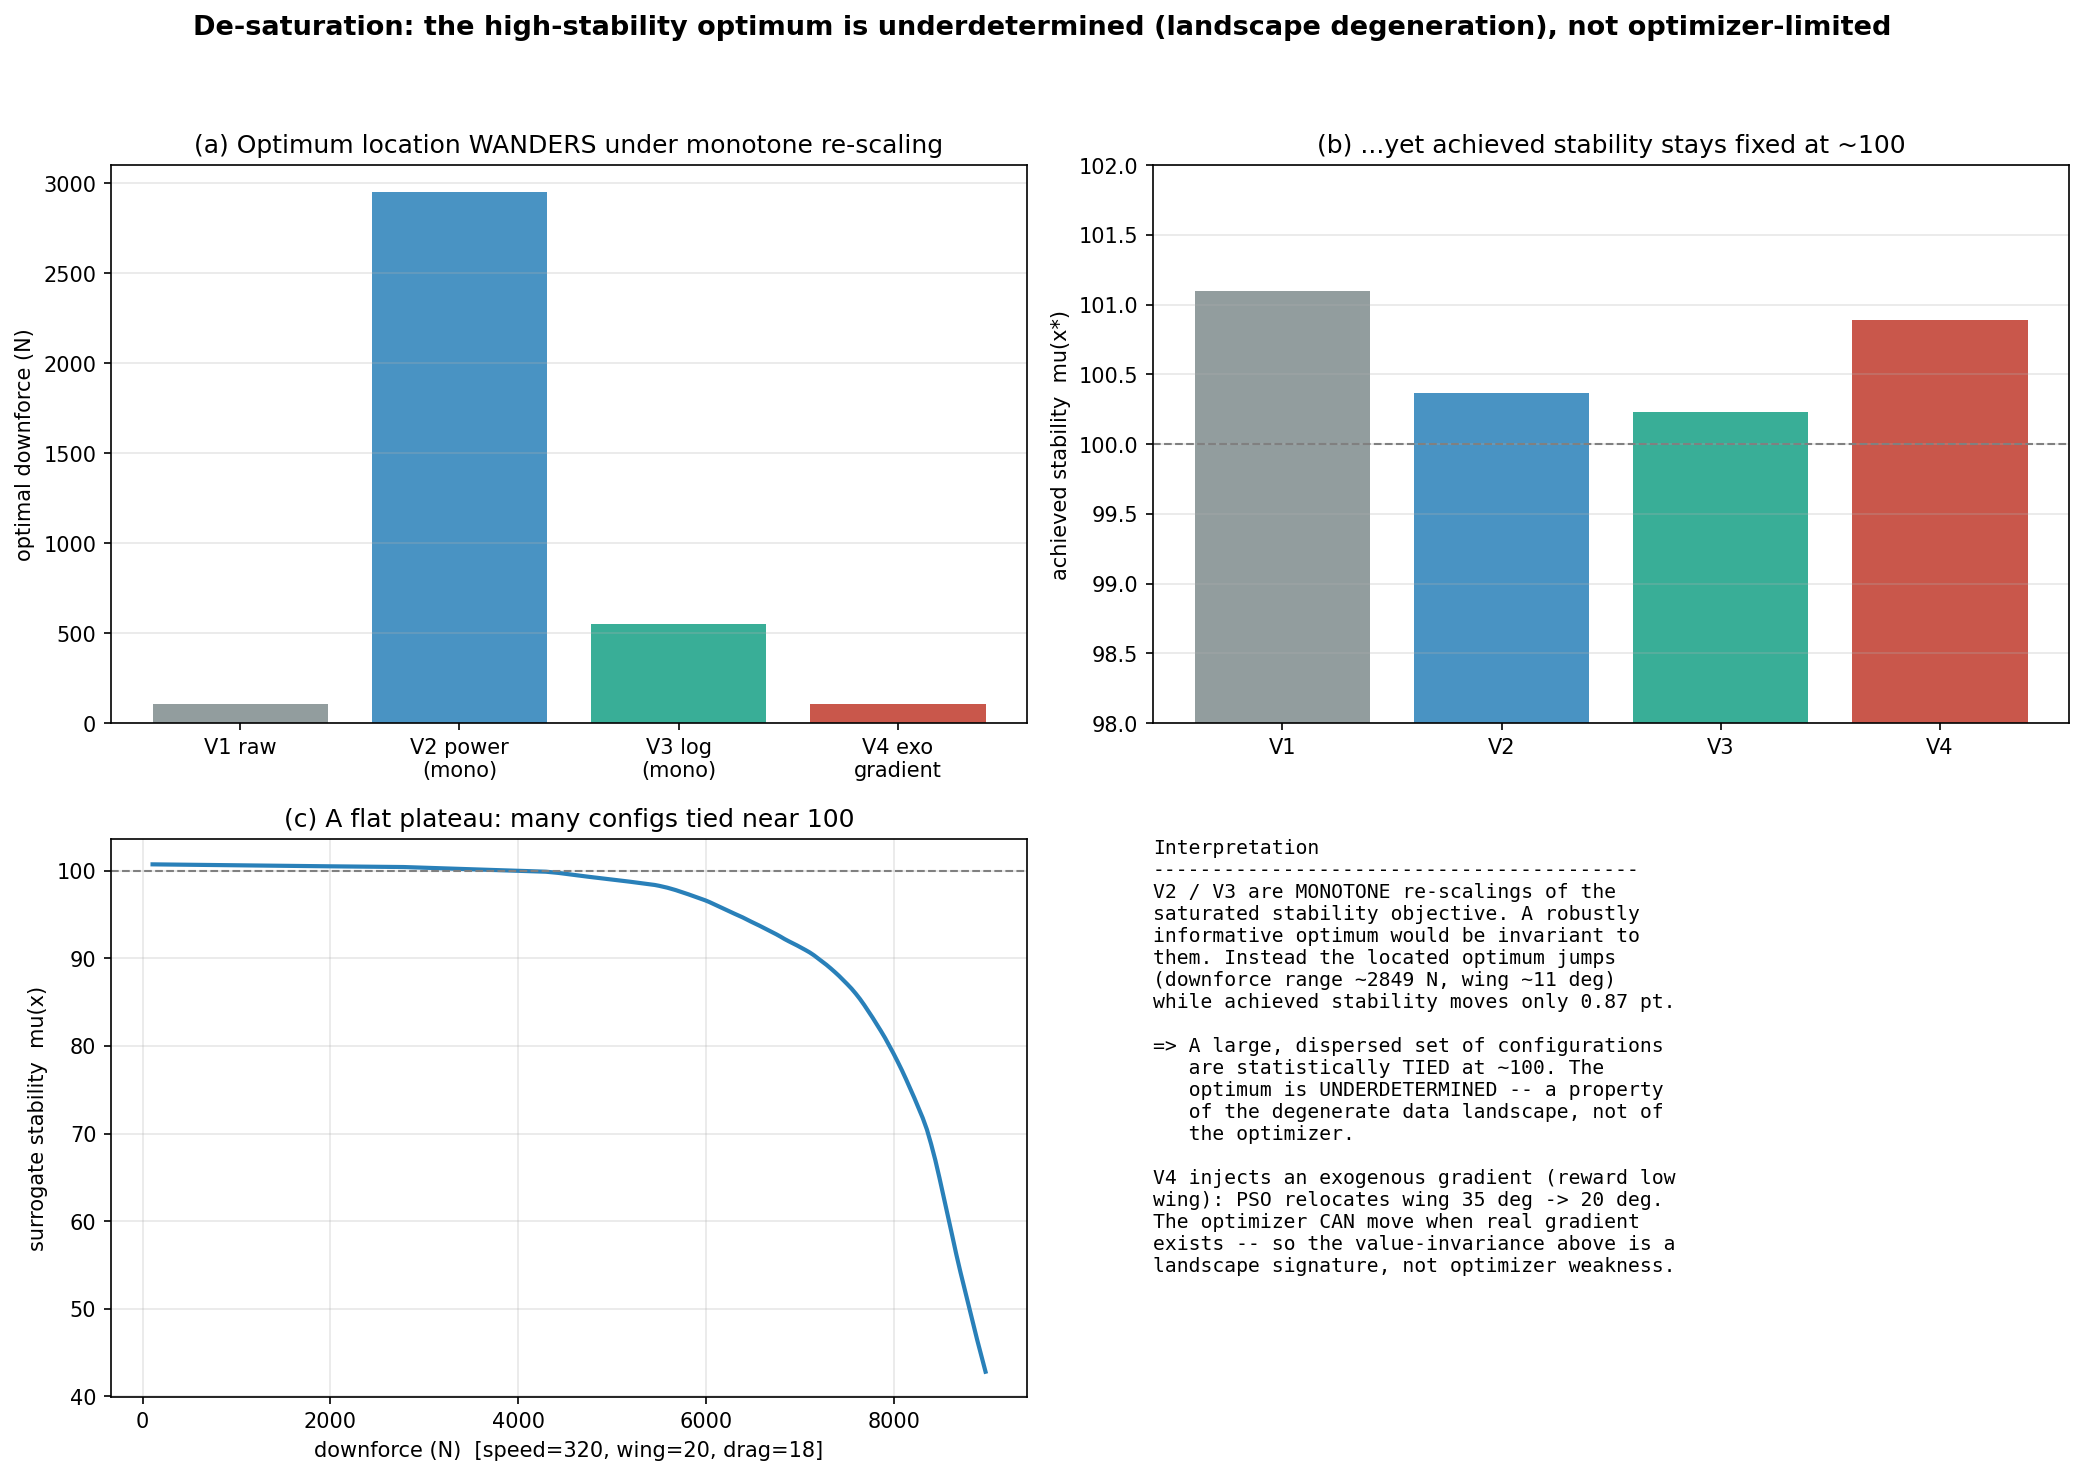
\includegraphics[width=0.95\textwidth]{figures/19_desaturation.png}
\caption{去饱和实验：不同目标变换下的最优解}
\label{fig:desat}
\end{figure}

关键设计与结果（图~\ref{fig:desat}）：
\begin{enumerate}
    \item \textbf{单调再标度（V2 幂变换、V3 对数变换）}：一个稳健的最优解
        应对单调变换不变。然而实测最优解大幅移动
        （下压力跨度 $\approx2849$ N、翼角跨度 $\approx10.7^\circ$），
        而达到的稳定性几乎不变（极差仅 $0.87$，均 $\approx100$）。
        这表明在饱和盆地内存在一大片几何上分散却统计上接近的配置，
        最优解处于\emph{欠定}状态，其位置更多与景观结构相关。
    \item \textbf{注入外生梯度（V4：奖励低翼角）}：在给出真实梯度后，
        PSO 将翼角从 $35^\circ$ 重新定位到 $20^\circ$。
        这表明优化器有能力移动解；因此前述对单调变换的价值不变性
        与景观退化的解释更一致，而非优化器能力不足。
\end{enumerate}

这与多目标加权使\emph{复合适应度}产生区分的现象相互印证
（多目标注入了 efficiency/power 的外生竞争梯度），
但该梯度仍不足以使 wing/drag 子空间的解分化（该子空间的退化未被打破）。

\subsection{综合解释：一种一致性的解释框架}

景观退化为前述各项异常提供了一种一致性的解释框架：
\begin{itemize}
    \item \textbf{异常一（预测越过 100）}：饱和盆地边缘的外推使代理输出越界，
        被 $\sigma$ 惩罚抑制（第~\ref{sec:risk}~节）；
    \item \textbf{异常二（算法同解，极差 0.15）}：退化景观下不同优化器均收敛到同一平坦盆地，
        更换算法不改变结果，SA 的随机游走甚至无法收敛；
    \item \textbf{异常三（场景/权重同解）}：可达解集合被 $r=0.895$ 共线收窄、
        被饱和抹平区分度，权重敏感性实验显示偏好几乎无法移动解（第~\ref{sec:converge}~节）；
    \item \textbf{DRS 失效}：数据生成器未编码 DRS 的差异化气动影响，其边际贡献接近零。
\end{itemize}

\begin{chapterquestion}
\textbf{主要发现之一（Key Finding）}：景观退化与数据结构限制，与优化结果趋同现象高度一致。
在代理驱动优化中，寻优上限受数据分布与景观结构约束；
当 86\% 样本趋于饱和、关键变量高度共线时，不同优化器均收敛到相近的平台解。
\end{chapterquestion}

\subsection{辅助解释：SHAP 的定位与限定}\label{subsec:shap}

SHAP 与排列重要性在本文中仅作为\textbf{辅助解释模块}，不承担核心论证。

\begin{figure}[H]
\centering
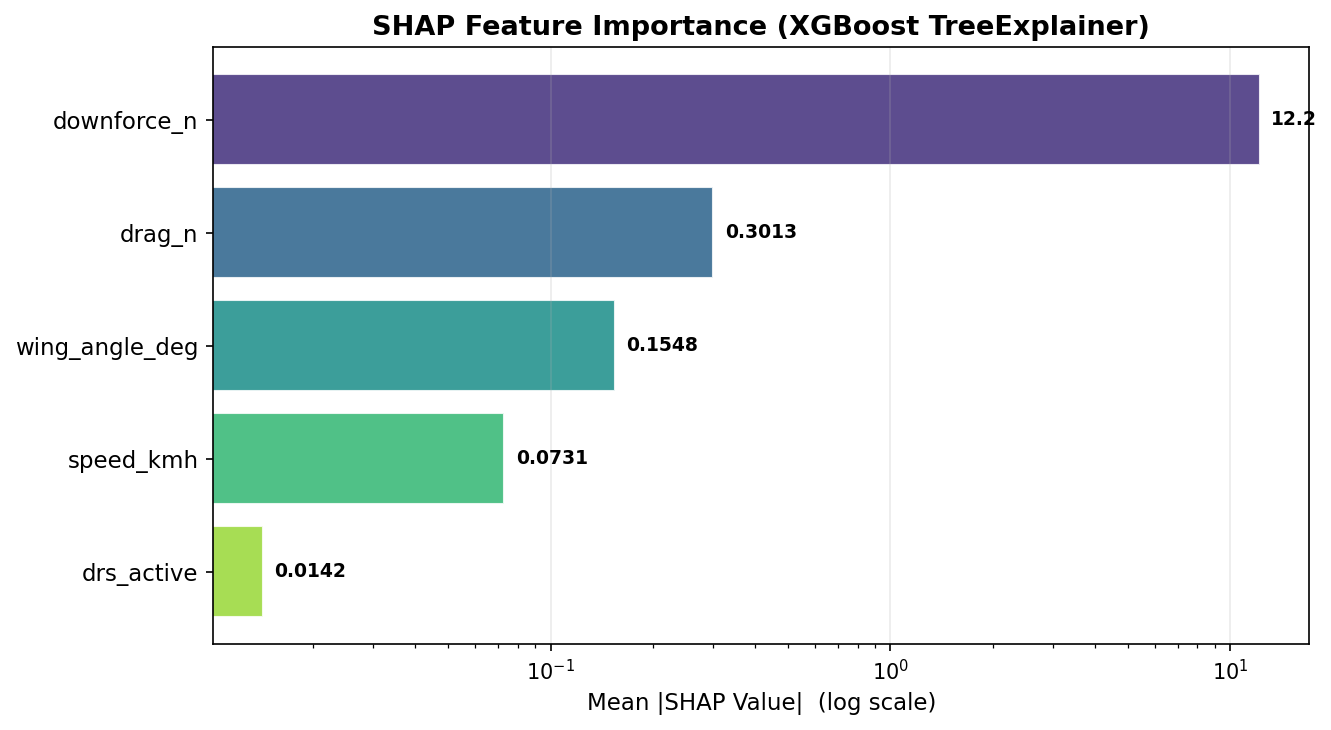
\includegraphics[width=0.72\textwidth]{figures/08_shap_summary.png}
\caption{SHAP 全局特征重要性（基于 XGBoost）}
\label{fig:shap}
\end{figure}

需特别限定：SHAP 反映的是模型决策中的\emph{统计关联}，而非\emph{物理因果}；
在 downforce 与 drag 共线（$r=0.895$）的情形下，
模型可能将 drag 的部分预测信息归因至 downforce。
因此"downforce 主导"应理解为该特征空间下的相对重要性，
而非各特征在物理层面的独立因果贡献。这一限定与景观退化的判断相互一致。
